\documentclass[conference]{IEEEtran}
\IEEEoverridecommandlockouts

\usepackage{cite}
\usepackage{amsmath,amssymb,amsfonts}
\usepackage{graphicx}
\usepackage{textcomp}
\usepackage{xcolor}
\usepackage{booktabs}
\usepackage{array}
\usepackage{multirow}
\usepackage[utf8]{inputenc}
\usepackage[T1]{fontenc}

\def\BibTeX{{\rm B\kern-.05em{\sc i\kern-.025em b}\kern-.08em
    T\kern-.1667em\lower.7ex\hbox{E}\kern-.125emX}}

\begin{document}

\title{Utilização de Modelos Classificadores para\\
Identificação de Área Queimada}

\author{
  \IEEEauthorblockN{Ryan\IEEEauthorrefmark{1},
                    Matheus V.~M.~Sales\IEEEauthorrefmark{1},
                    Pedro\IEEEauthorrefmark{1},
                    Abner\IEEEauthorrefmark{1}}
  \IEEEauthorblockA{\IEEEauthorrefmark{1}
    \textit{Instituto Nacional de Pesquisas Espaciais (INPE)}\\
    São José dos Campos, Brasil
  }
}

\maketitle

%---------------------------------------------------------------------
\begin{abstract}
Este trabalho compara seis abordagens de aprendizado de máquina para
detecção automática de áreas queimadas em imagens Landsat~8/9 (Cerrado
brasileiro, agosto de 2024): K-Nearest Neighbors (KNN), SVM Linear,
SVM com kernel RBF, Multilayer Perceptron (MLP), \textit{Self-Organizing
Map} (SOM) e Random Forest (RF). Os modelos supervisionados utilizam
até dez atributos espectrais multitemporais — bandas B4, B5, B7, NDVI e
NBR nas datas pré e pós-incêndio. São abordados três desafios
metodológicos recorrentes: desbalanceamento de classes (até 33:1),
autocorrelação espacial entre amostras e circularidade entre atributos
e rótulos (\textit{feature leakage}). A SVM~RBF obteve o melhor
desempenho nos testes cegos ($F_1 > 98\%$, AUC-ROC~$= 1{,}000$, com
apenas 105 vetores de suporte). O RF com validação por blocos espaciais
forneceu a avaliação mais rigorosa ($F_2 = 0{,}472$ em generalização
cross-cena). A SOM detectou $\approx$154~mil hectares sem nenhum rótulo.
O KNN apresentou 73\% de acurácia interna, mas apenas 9\% de Precision
ao generalizar para nova cena, evidenciando forte dependência da cena
de treinamento.
\end{abstract}

\begin{IEEEkeywords}
área queimada, Landsat, sensoriamento remoto, KNN, SVM, MLP, SOM,
Random Forest, desbalanceamento, leakage, validação espacial, Optuna.
\end{IEEEkeywords}

%=====================================================================
\section{Introdução}

O mapeamento de áreas queimadas é uma demanda crescente para o
monitoramento ambiental, gestão de risco e estimativas do ciclo do
carbono. No Brasil, a frequência de queimadas nos biomas Cerrado e
Amazônia reforça a necessidade de métodos automatizados sobre imagens
Landsat~8/9 (resolução espacial de 30~m, revisita $\approx$8~dias)~\cite{b1}.

Abordagens clássicas baseadas em limiar espectral como o dNBR~\cite{b2}
são operacionalmente simples mas dependem de calibração manual e não
exploram a combinação de múltiplas bandas. Algoritmos de aprendizado de
máquina oferecem alternativas mais flexíveis, porém exigem atenção a
três problemas metodológicos frequentemente ignorados: (i)~\textbf{
desbalanceamento de classes} — pixels não queimados superam os queimados
em até 33:1; (ii)~\textbf{autocorrelação espacial} — pixels vizinhos
são estatisticamente dependentes, invalidando divisões aleatórias para
treino/teste; e (iii)~\textbf{leakage circular} — quando o índice que
gerou a máscara de referência é também usado como atributo, as métricas
atingem valores artificialmente perfeitos.

Este trabalho avalia e compara seis algoritmos, discutindo como cada
um endereça — ou falha em endereçar — esses desafios.

%=====================================================================
\section{Referencial Teórico}

\subsection{Índices Espectrais}

O NBR (\textit{Normalized Burn Ratio}) e o NDVI (\textit{Normalized
Difference Vegetation Index}) quantificam, respectivamente, a degradação
por queima e a cobertura vegetal:

\begin{equation}
  \mathrm{NBR} = \frac{\rho_\text{NIR}-\rho_\text{SWIR}}
                      {\rho_\text{NIR}+\rho_\text{SWIR}}, \quad
  \mathrm{NDVI} = \frac{\rho_\text{NIR}-\rho_\text{Red}}
                       {\rho_\text{NIR}+\rho_\text{Red}}
  \label{eq:indices}
\end{equation}

A diferença temporal dNBR (pré $-$ pós) sinaliza cicatrizes de queimada;
valores altos de dNBR indicam destruição de vegetação e exposição de
carbono~\cite{b2}.

\subsection{Algoritmos}

\textbf{KNN}: classifica cada pixel pela classe majoritária entre seus
$K$ vizinhos mais próximos; não aprende fronteira explícita.

\textbf{SVM}~\cite{b7}: encontra o hiperplano de margem máxima entre
classes. O kernel RBF extende a separação a fronteiras não-lineares:
$K(\mathbf{x},\mathbf{x}') = \exp(-\gamma\|\mathbf{x}-\mathbf{x}'\|^2)$.

\textbf{MLP}~\cite{b9}: rede neural com camadas ocultas totalmente
conectadas, treinada por retropropagação com BatchNorm, Dropout e
Early Stopping.

\textbf{SOM}~\cite{b8}: rede não supervisionada que organiza neurônios
em grade~2D preservando a topologia do espaço de entrada; não utiliza
rótulos.

\textbf{RF}~\cite{b3}: ensemble de árvores de decisão com bootstrap
e seleção aleatória de atributos; fornece importância via impureza Gini.

\subsection{Estratégias de Desbalanceamento}

Quatro estratégias são avaliadas no RF: (i)~\textit{class\_weight=
balanced}, que penaliza erros na classe minoritária proporcionalmente
à razão de classes; (ii)~\textit{undersampling} aleatório da classe
majoritária; (iii)~SMOTE~\cite{b5}, que gera amostras sintéticas por
interpolação entre vizinhos; e (iv)~SMOTETomek, que combina SMOTE com
remoção de pares de fronteira ruidosos.

%=====================================================================
\section{Dados e Área de Estudo}

\subsection{Cenas Landsat}

Foram utilizadas três cenas Landsat Coleção~2 L2SP (reflectância de
superfície, agosto de 2024) cobrindo o Cerrado brasileiro:

\begin{itemize}
  \item \textbf{221/074} — LC08, 28/08: treinamento principal;
  \item \textbf{220/075} — LC09, 29/08: treinamento secundário e teste
        de generalização cross-cena;
  \item \textbf{222/074} — LC09, 27/08: teste cego exclusivo (SVM~RBF
        e MLP).
\end{itemize}

Cada cena possui $\approx$40~milhões de pixels válidos após
mascaramento de nuvens e bordas. A Fig.~\ref{fig:cenas} apresenta as
composições falsa-cor, dNBR e máscaras de referência.

\begin{figure}[!t]
  \centering
  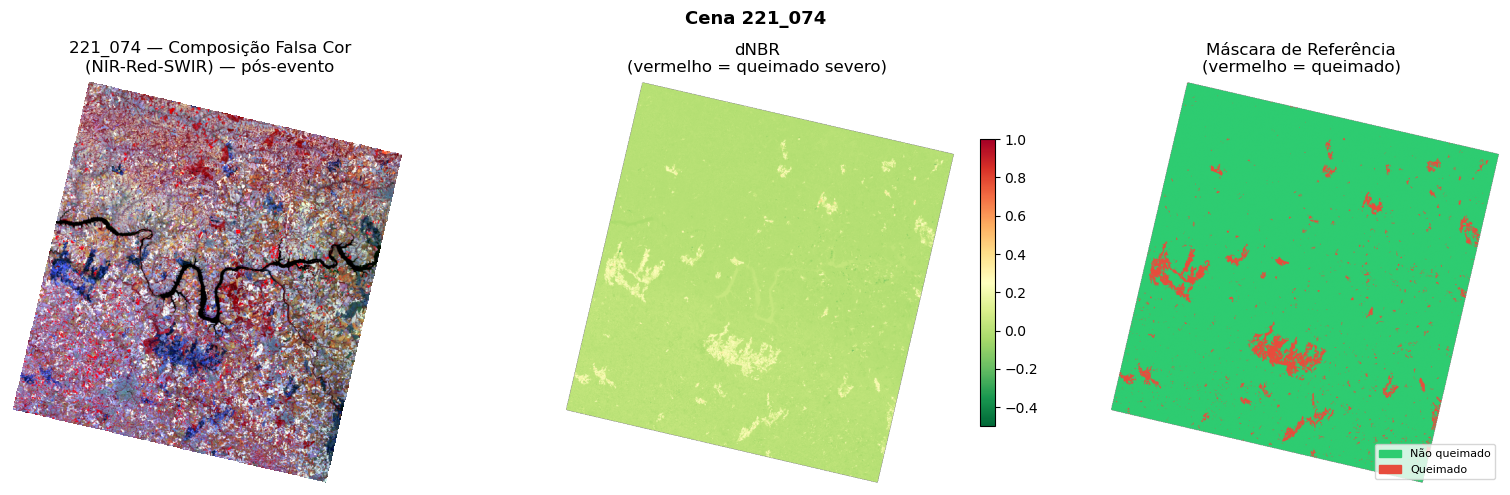
\includegraphics[width=\columnwidth]{figs/rf/fig_cena_221074.png}\\[2pt]
  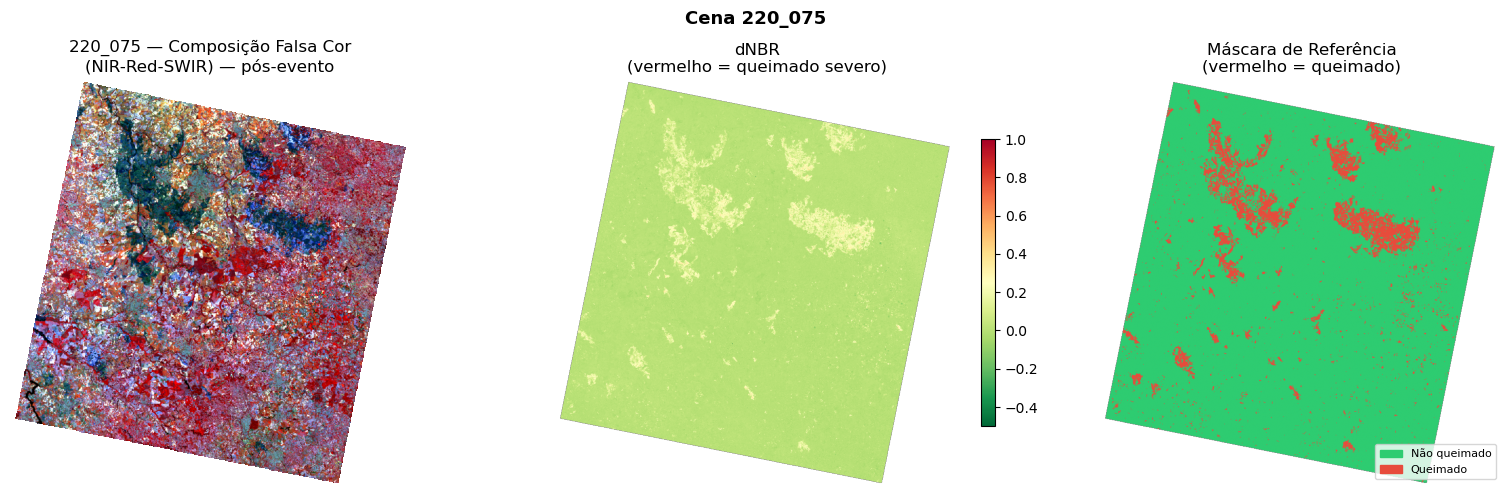
\includegraphics[width=\columnwidth]{figs/rf/fig_cena_220075.png}
  \caption{Cenas 221/074 (cima) e 220/075 (baixo): composição
           falsa-cor NIR-Red-SWIR (esq.), dNBR (centro) e máscara
           de referência (dir.). Vermelho = área queimada.}
  \label{fig:cenas}
\end{figure}

\subsection{Atributos de Entrada}

A Tabela~\ref{tab:features} descreve os atributos espectrais utilizados.
Os modelos com 10~atributos extraem cinco valores da imagem pré-queimada
e cinco da pós-queimada. Os índices dNBR e dNDVI foram \textbf{excluídos}
dos modelos supervisionados (exceto KNN): a máscara de referência foi
gerada com limiar dNBR~$>$~0,65, de modo que incluí-los criaria
circularidade direta entre atributo e rótulo.

\begin{table}[!t]
  \caption{Atributos espectrais e sua relevância para detecção}
  \label{tab:features}
  \centering
  \begin{tabular}{lll}
    \toprule
    \textbf{Atributo} & \textbf{O que mede} & \textbf{Relevância} \\
    \midrule
    B4 (Red)   & Reflectância vermelha    & Aumenta após queima \\
    B5 (NIR)   & Infravermelho próximo    & Cai com destruição vegetal \\
    B7 (SWIR2) & IV onda curta            & Alto em solo exposto \\
    NDVI       & Cobertura vegetal        & Queda = perda de cobertura \\
    NBR        & Índice de queimada       & Principal discriminador \\
    \bottomrule
    \multicolumn{3}{l}{\footnotesize Cada atributo extraído em 2 datas:
      pré e pós $= 10$~features total.}
  \end{tabular}
\end{table}

\subsection{Desbalanceamento de Classes}

A proporção de área queimada varia entre 2,96\% (222/074) e 7,9\%
(220/075), configurando razão de até 33:1 entre classes. Esse
desbalanceamento afeta diretamente a capacidade de todos os modelos
supervisionados de detectar a classe minoritária.

%=====================================================================
\section{Modelos e Metodologia}

\subsection{KNN ($K=5$)}

Amostras coletadas manualmente via QGIS em dois shapefiles de pontos
(\texttt{pontos\_mistos.shp} e \texttt{pontos\_nao\_qmd.shp}). Atributos:
dNBR, dNBRSWIR e dNDVI normalizados por \texttt{StandardScaler}. Divisão
aleatória 70/30 para treino e teste interno; generalização avaliada em
cena Landsat independente.

\subsection{SVM Linear}

\texttt{LinearSVC} com \texttt{class\_weight='balanced'} e
\texttt{StandardScaler}. Apenas dois atributos: NDVI pré e pós-queimada.
Amostragem balanceada com 25~000~pixels por classe. Treinamento em cenas
220/075 e 221/074; avaliação na cena 222/074.

\subsection{SVM com Kernel RBF}

Dez atributos, treinamento exclusivo na cena 220/075, avaliação cega em
221/074 e 222/074. Hiperparâmetros $C$ e $\gamma$ otimizados por
\textbf{Optuna} (50~tentativas, TPE Sampler) maximizando $F_1$ em
validação cruzada.

\subsection{MLP}

PyTorch, 2~camadas~$\times$~64~neurônios, BatchNorm~+~ReLU~+~Dropout
(0,256), Adam ($\alpha=10^{-3}$), CrossEntropyLoss com pesos de classe
e Early Stopping (paciência~10). Optuna (5~tentativas) ajustou
hiperparâmetros. Treinamento balanceado (100k~pixels/classe) em cenas
220/075 e 221/074; validação Stratified 5-Fold CV; teste cego em 222/074
(40,3~M pixels, 2,96\% queimada).

\subsection{SOM}

Grade $15\times15$~neurônios otimizada por Optuna (20~tentativas) via
função de score que combina Quantization Error (QE) e Topographic Error
(TE): $\text{Score} = 0{,}7 \cdot \text{QE} + 0{,}3 \cdot \text{TE}$.
Após treinamento, K-Means agrupa os neurônios em 3~clusters; rótulos
semânticos são atribuídos por heurística espectral ($\Delta$NBR alto
$\to$ Queimada; NIR baixo + NDVI negativo $\to$ Água). Aplicada
exclusivamente à cena 221/074 com 7~atributos.

\subsection{Random Forest}

Dez atributos, quatro estratégias de desbalanceamento comparadas.
Hiperparâmetros por RandomizedSearchCV (30~iterações, 5-fold CV,
critério $F_1$): \texttt{max\_depth=30}, \texttt{max\_features=sqrt},
\texttt{min\_samples\_leaf=11}, \texttt{n\_estimators=171}.

\textbf{Validação por blocos espaciais} ($4\times4$, 16~blocos, 25\%
para teste): pixels do mesmo bloco geográfico ficam no mesmo conjunto,
eliminando autocorrelação espacial~\cite{b4}.

O threshold de decisão é otimizado pela maximização de $F_2$ na curva
Precision-Recall:

\begin{equation}
  \tau^* = \underset{\tau}{\arg\max}\;
  F_2(\tau) = \frac{5 P(\tau) R(\tau)}{4 P(\tau) + R(\tau)}
  \label{eq:f2}
\end{equation}

A Fig.~\ref{fig:rf_blocos} ilustra a divisão por blocos aplicada à
cena 221/074.

\begin{figure}[!t]
  \centering
  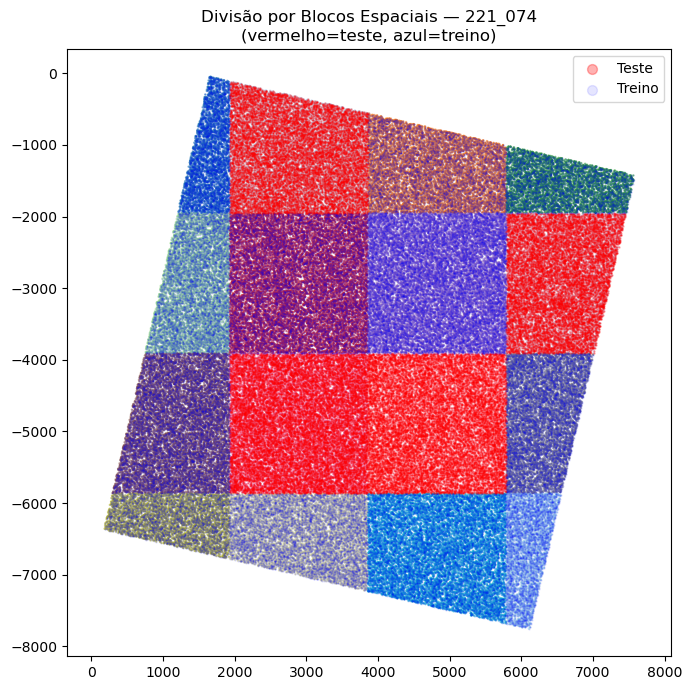
\includegraphics[width=0.9\columnwidth]{figs/rf/fig_blocos_espaciais.png}
  \caption{Divisão por blocos espaciais RF ($4\times4$, cena 221/074).
           Vermelho = blocos de teste; azul = treino.}
  \label{fig:rf_blocos}
\end{figure}

%=====================================================================
\section{Resultados}

\subsection{KNN}

Internamente, o modelo atingiu acurácia de 73\% e F1~$= 0{,}74$
para a classe queimada. Ao generalizar para nova cena, a Precision caiu
de 71\% para apenas 9\% e o F1 de 0,74 para 0,17
(Tabela~\ref{tab:knn}). A Fig.~\ref{fig:knn} mostra visualmente
a forte superestimação de área queimada na nova cena.

\begin{table}[!t]
  \caption{KNN ($K=5$) — métricas internas vs.\ nova cena}
  \label{tab:knn}
  \centering
  \setlength{\tabcolsep}{4pt}
  \begin{tabular}{lcccc}
    \toprule
    \textbf{Conjunto} & \textbf{Acc.} & \textbf{Prec.} & \textbf{Recall} & \textbf{F1} \\
    \midrule
    Interno (30\%)      & 0,73 & 0,71 & 0,77 & 0,74 \\
    Nova cena (cego)    & 0,69 & 0,09 & 0,82 & 0,17 \\
    \bottomrule
  \end{tabular}
\end{table}

\begin{figure}[!t]
  \centering
  \begin{minipage}[b]{0.48\columnwidth}
    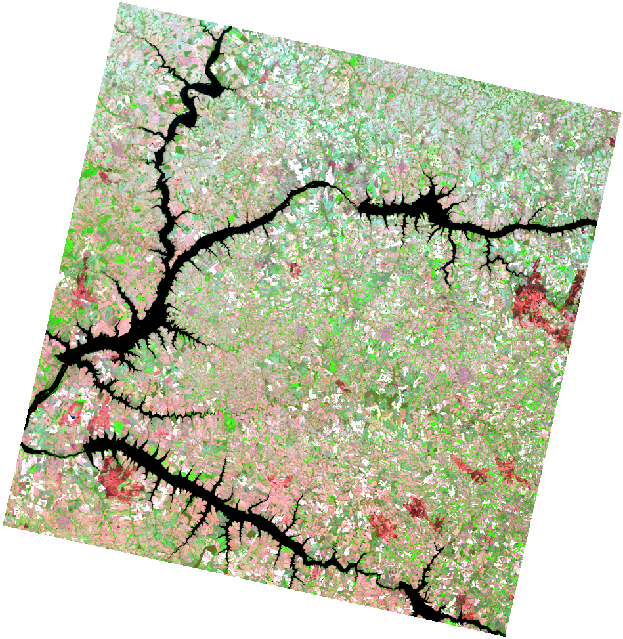
\includegraphics[width=\textwidth]{imgs_knn/cena_treinamento.png}
    \caption*{(a) Cena treino}
  \end{minipage}
  \hfill
  \begin{minipage}[b]{0.48\columnwidth}
    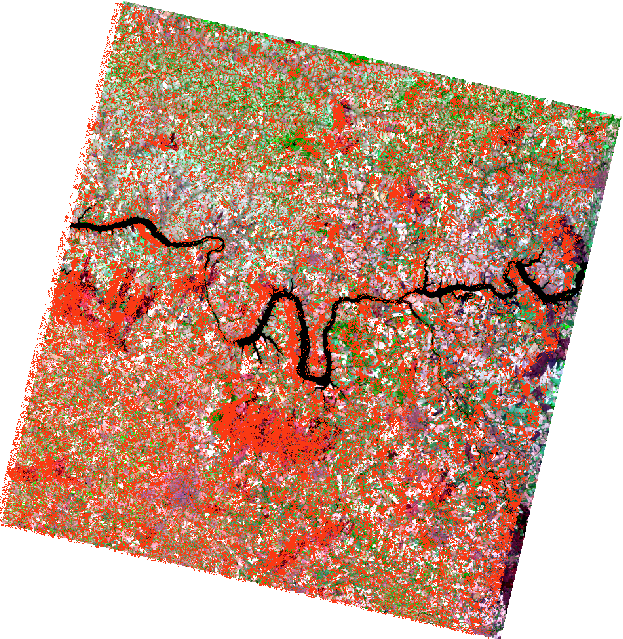
\includegraphics[width=\textwidth]{imgs_knn/cena_teste_classificada.png}
    \caption*{(b) Classificação nova cena}
  \end{minipage}
  \caption{KNN: (a)~cena de treinamento e (b)~resultado da classificação
           em nova cena. A superestimação (excesso de vermelho) evidencia
           a alta taxa de falsos positivos.}
  \label{fig:knn}
\end{figure}

\subsection{SVM Linear}

Com apenas NDVI pré e pós-queimada como atributos, o modelo atingiu
Recall~$= 83{,}4\%$ na cena 222/074, mas Precision de apenas 14\%
(Tabela~\ref{tab:svm_linear}). O elevado número de falsos positivos
reflete a semelhança espectral entre solo exposto, pastagens degradadas
e cicatrizes de queimada no espaço bidimensional de NDVI.

\begin{table}[!t]
  \caption{SVM Linear — cena 222/074 (teste)}
  \label{tab:svm_linear}
  \centering
  \begin{tabular}{ccccc}
    \toprule
    \textbf{Acc.} & \textbf{Prec.} & \textbf{Recall} & \textbf{F1} & \textbf{IoU} \\
    \midrule
    80,1\% & 14,0\% & 83,4\% & 24,0\% & 13,7\% \\
    \bottomrule
  \end{tabular}
\end{table}

\subsection{SVM com Kernel RBF}

O modelo generalizou com excelência para ambas as cenas de teste cego,
atingindo $F_1 > 98\%$ e AUC-ROC~$= 1{,}000$ em todas as avaliações
(Tabela~\ref{tab:svm_rbf}). Apenas \textbf{105 vetores de suporte}
foram necessários sobre 50~mil amostras de treino — número reduzido
que confirma a forte separabilidade espectral das classes no espaço de
10~atributos. A Fig.~\ref{fig:svm_rbf_optuna} mostra a convergência da
busca de hiperparâmetros pelo Optuna.

\begin{table}[!t]
  \caption{SVM RBF — desempenho em todos os conjuntos}
  \label{tab:svm_rbf}
  \centering
  \setlength{\tabcolsep}{3.5pt}
  \begin{tabular}{lcccc}
    \toprule
    \textbf{Conjunto} & \textbf{Acc.} & \textbf{Prec.} & \textbf{Recall} & \textbf{F1} \\
    \midrule
    Treino (50k amostras)    & 99,96\% & 98,69\% & 100,00\% & 99,34\% \\
    Validação (12M pixels)   & 99,85\% & 98,40\% &  99,76\% & 99,07\% \\
    Cego 221/074 (40M px)    & 99,91\% & 98,60\% &  99,64\% & \textbf{99,12\%} \\
    Cego 222/074 (40M px)    & 99,88\% & 96,83\% &  99,30\% & \textbf{98,05\%} \\
    \bottomrule
    \multicolumn{5}{l}{AUC-ROC $= 1{,}000$ em todos os conjuntos.}
  \end{tabular}
\end{table}

\begin{figure}[!t]
  \centering
  
\includegraphics[width=\columnwidth]{figs/svm_rbf/fig_optuna.png}
  \caption{Busca de hiperparâmetros SVM RBF (Optuna, 50 tentativas):
           convergência do $F_1$ (esq.) e espaço $C \times \gamma$
           colorido pelo $F_1$ obtido (dir.).}
  \label{fig:svm_rbf_optuna}
\end{figure}

\begin{figure}[!t]
  \centering
  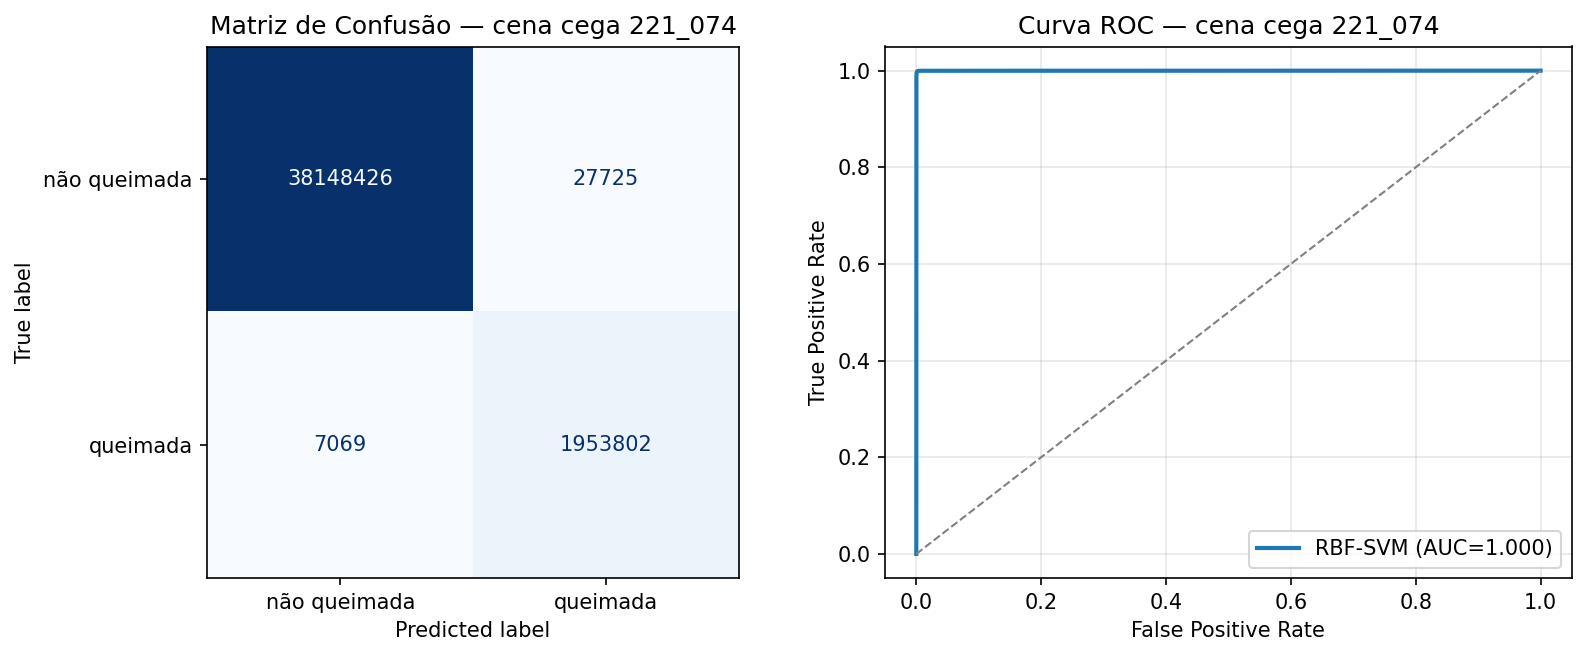
\includegraphics[width=\columnwidth]{figs/svm_rbf/fig_cm_221.png}\\[3pt]
  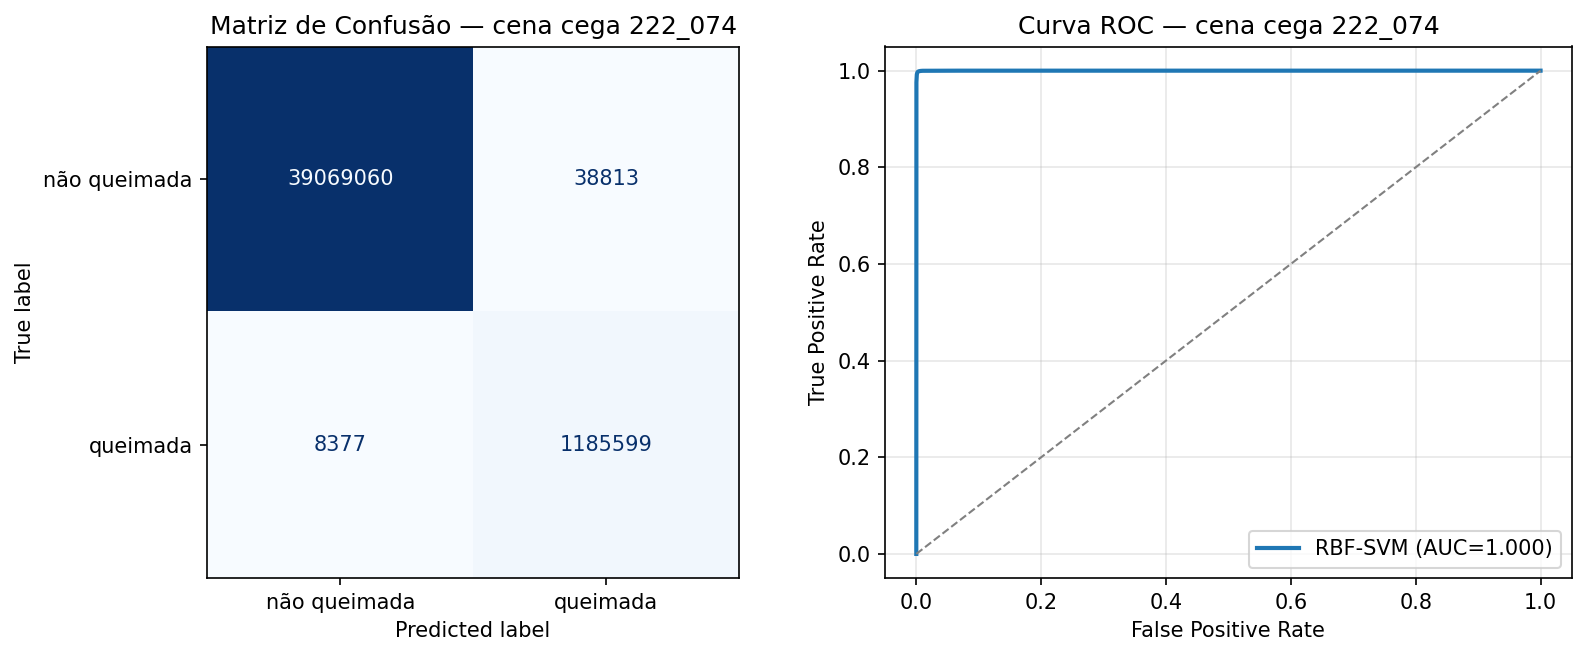
\includegraphics[width=\columnwidth]{figs/svm_rbf/fig_cm_222.png}
  \caption{SVM RBF: CM e curva ROC para cena 221/074 (cima) e 222/074
           (baixo). AUC-ROC~$= 1{,}000$ em ambas.}
  \label{fig:svm_rbf_cm}
\end{figure}

\subsection{MLP}

A validação cruzada 5-fold sobre 400k~pixels balanceados atingiu
$F_1 = 0{,}722 \pm 0{,}002$ e AUC~$= 0{,}812 \pm 0{,}002$
(Tabela~\ref{tab:mlp_cv}). O baixo desvio padrão entre folds confirma
estabilidade e ausência de overfitting.

\begin{table}[!t]
  \caption{MLP — Stratified 5-Fold CV (cenas 220/075 + 221/074)}
  \label{tab:mlp_cv}
  \centering
  \setlength{\tabcolsep}{4pt}
  \begin{tabular}{cccccc}
    \toprule
    \textbf{Fold} & \textbf{Acc.} & \textbf{Prec.} & \textbf{Recall}
                  & \textbf{F1} & \textbf{AUC} \\
    \midrule
    1 & 0,731 & 0,745 & 0,701 & 0,723 & 0,810 \\
    2 & 0,732 & 0,756 & 0,684 & 0,718 & 0,811 \\
    3 & 0,732 & 0,747 & 0,702 & 0,724 & 0,811 \\
    4 & 0,735 & 0,759 & 0,688 & 0,722 & 0,814 \\
    5 & 0,734 & 0,756 & 0,691 & 0,722 & 0,814 \\
    \midrule
    \textbf{Méd.} & \textbf{0,733} & \textbf{0,753} & \textbf{0,693}
                  & \textbf{0,722} & \textbf{0,812} \\
    \textbf{DP}   & 0,002 & 0,006 & 0,008 & 0,002 & 0,002 \\
    \bottomrule
  \end{tabular}
\end{table}

No teste cego (222/074, 40,3~M pixels), o AUC permaneceu em 0,830, mas
a Precision caiu para 11,6\% com threshold~$= 0{,}5$ — consequência
do treino balanceado 50/50 aplicado a uma cena 97:3
(Tabela~\ref{tab:mlp_test}).

\begin{table}[!t]
  \caption{MLP — CV vs.\ teste cego 222/074}
  \label{tab:mlp_test}
  \centering
  \setlength{\tabcolsep}{4pt}
  \begin{tabular}{lccccc}
    \toprule
    \textbf{Conjunto} & \textbf{Acc.} & \textbf{Prec.}
                      & \textbf{Recall} & \textbf{F1} & \textbf{AUC} \\
    \midrule
    CV (média)          & 0,733 & 0,753 & 0,693 & 0,722 & 0,812 \\
    Cego 222/074 (40M)  & 0,830 & 0,116 & 0,713 & 0,199 & 0,830 \\
    \bottomrule
  \end{tabular}
\end{table}

\begin{figure}[!t]
  \centering
  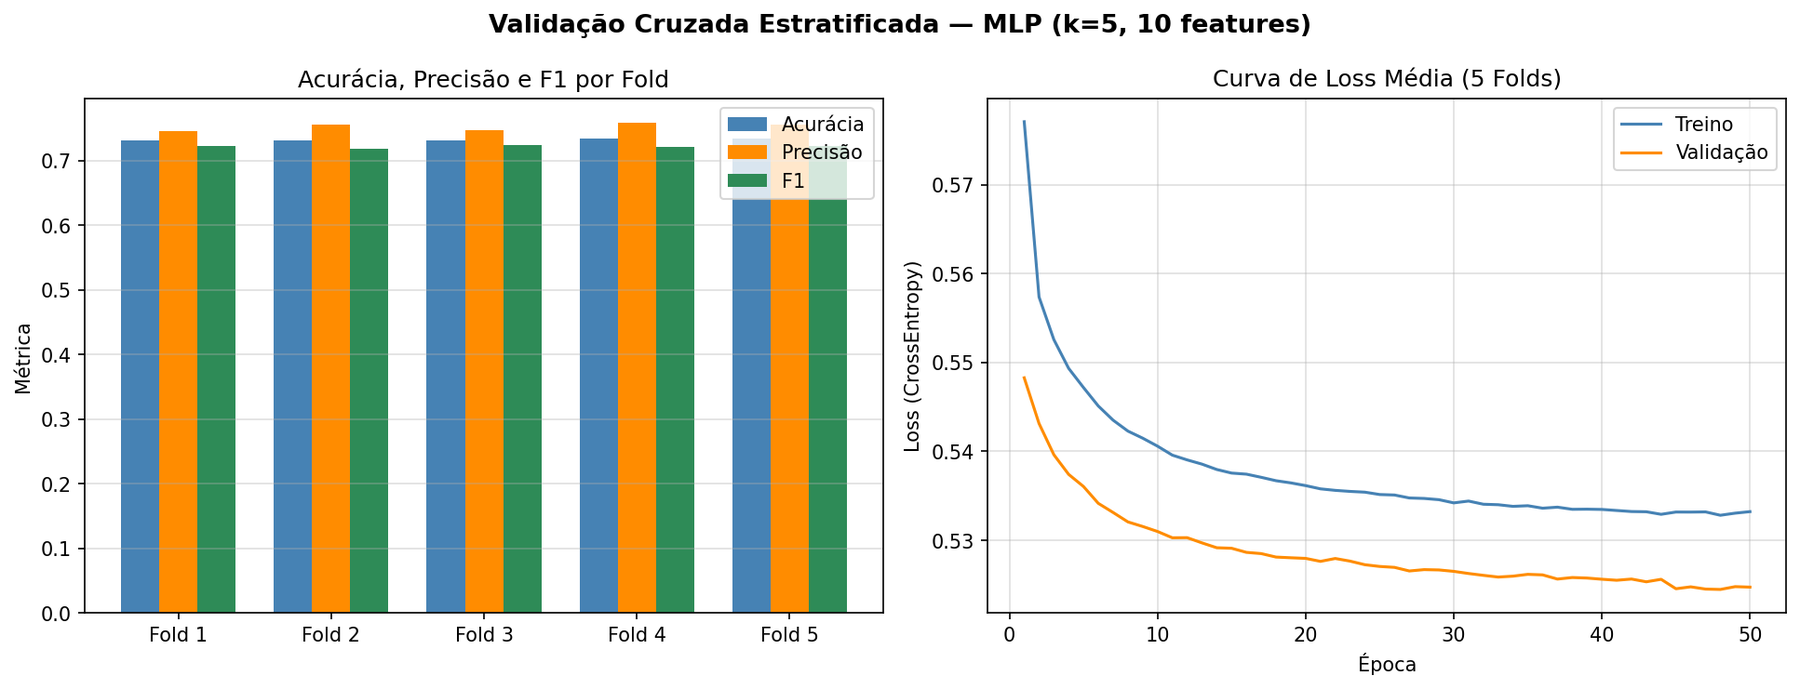
\includegraphics[width=\columnwidth]{figs/mlp/fig_curvas_val.png}
  \caption{MLP: métricas por fold (esq.) e curva de loss média dos
           5~folds (dir.). Convergência estável sem overfitting.}
  \label{fig:mlp_curvas}
\end{figure}

\subsection{SOM}

As métricas internas confirmam boa qualidade do mapeamento não
supervisionado (Tabela~\ref{tab:som}). A SOM detectou
$\approx$\textbf{154~mil hectares} de área queimada (~4,3\% da cena
221/074). A Fig.~\ref{fig:som} apresenta a grade topológica e o mapa
de classificação resultante.

\begin{table}[!t]
  \caption{SOM ($15\times15$) — métricas internas e área estimada}
  \label{tab:som}
  \centering
  \begin{tabular}{llr}
    \toprule
    \textbf{Métrica} & \textbf{Valor} & \textbf{Interpretação} \\
    \midrule
    Quantization Error & 0,572 & Boa representação dos pixels \\
    Topographic Error  & 0,133 & Vizinhança espacial preservada \\
    Silhouette         & 0,341 & Separabilidade aceitável \\
    \midrule
    Área queimada  & $\sim$154k~ha & 4,3\% da cena 221/074 \\
    Não queimada   & $\sim$3.322k~ha & 93\% da cena \\
    Água           & $\sim$97k~ha  & 2,7\% da cena \\
    \bottomrule
  \end{tabular}
\end{table}

\begin{figure}[!t]
  \centering
  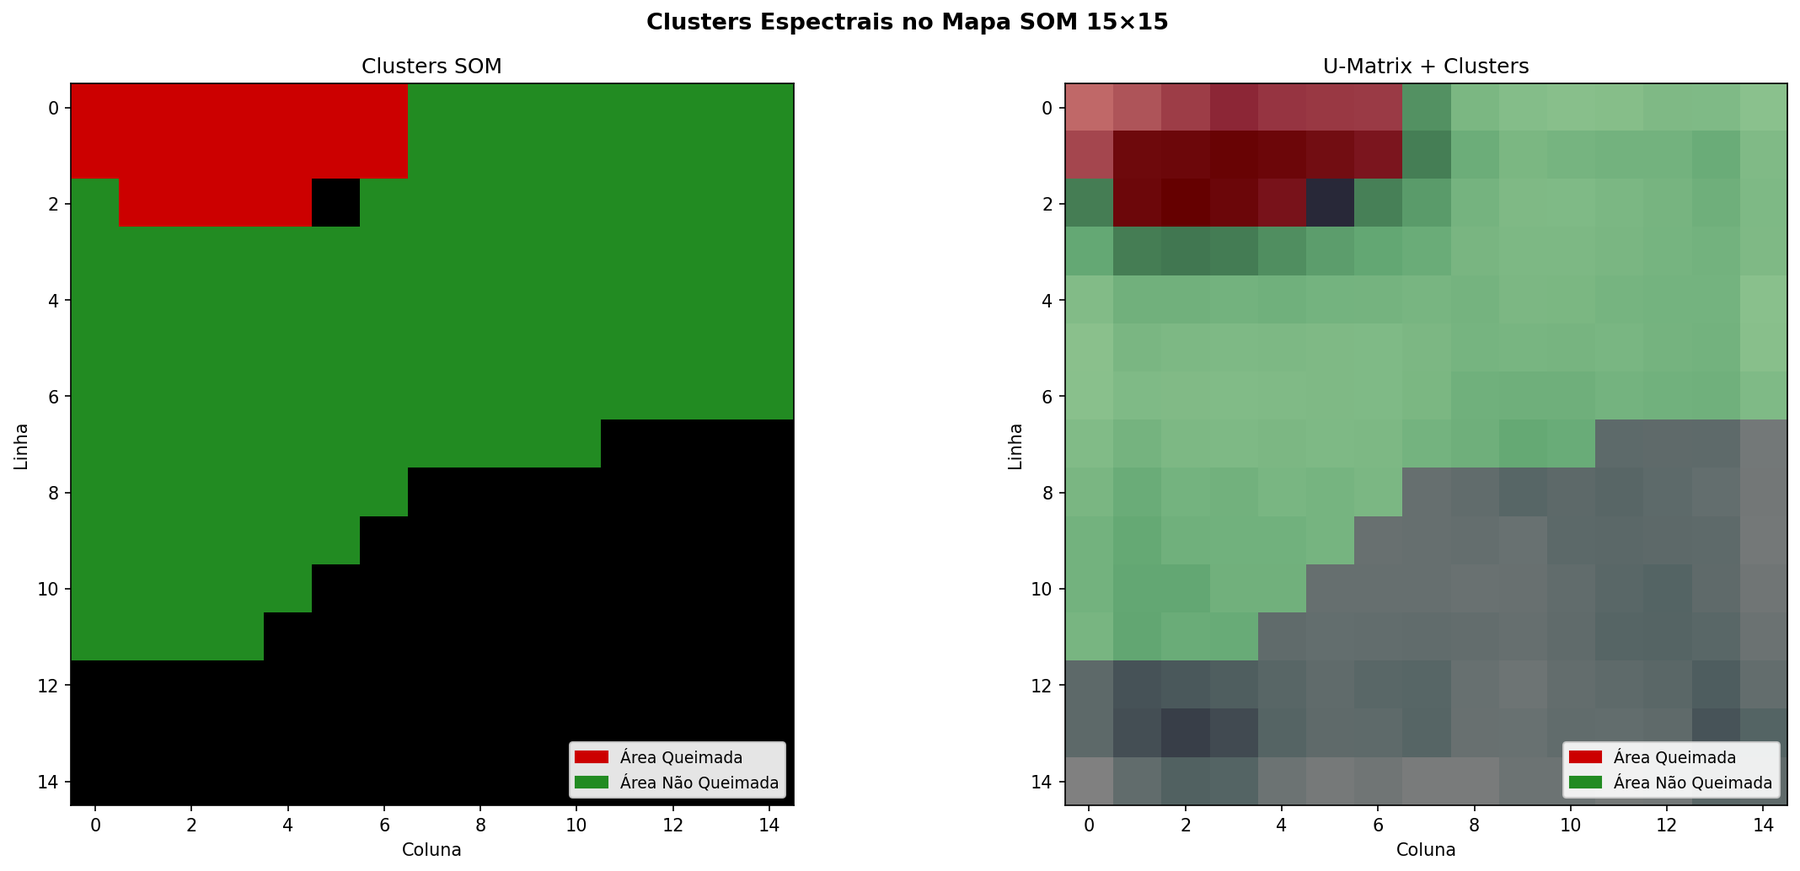
\includegraphics[width=\columnwidth]{figs/som/fig_clusters.png}\\[3pt]
  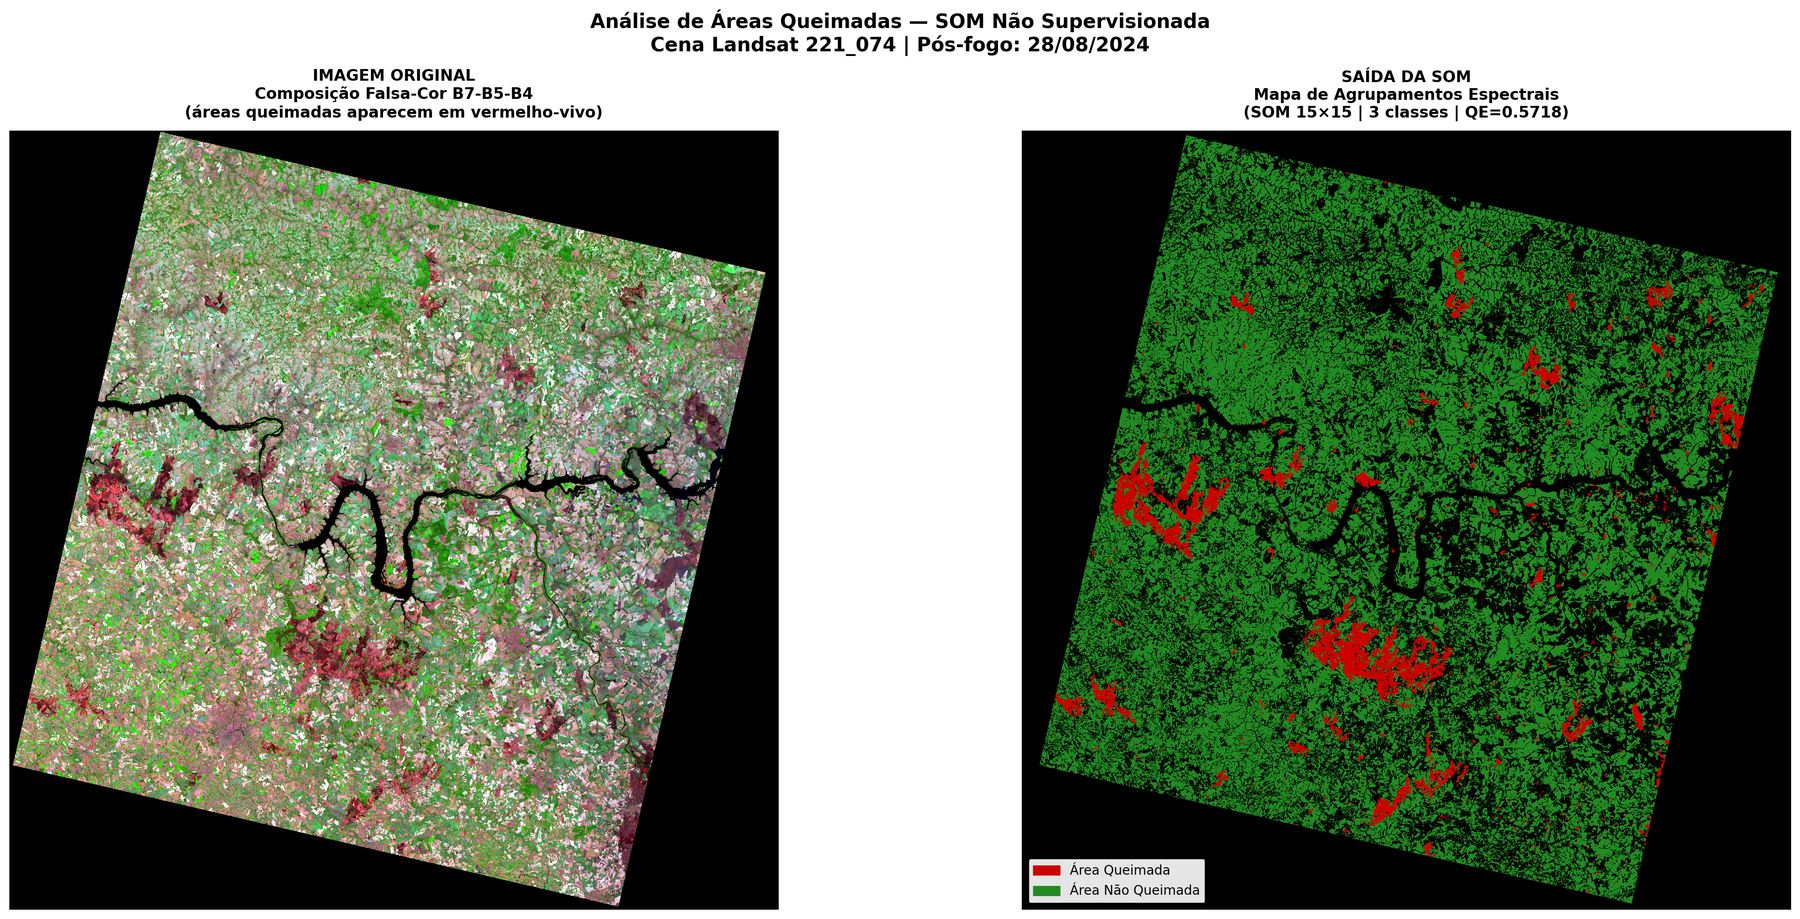
\includegraphics[width=\columnwidth]{figs/som/fig_mapa.png}
  \caption{SOM $15\times15$: grade com clusters K-Means e U-Matrix
           (cima); composição falsa-cor vs.\ mapa classificado (baixo).
           Cicatrizes detectadas sem nenhum rótulo.}
  \label{fig:som}
\end{figure}

\subsection{Random Forest}

\subsubsection{Estratégias de Desbalanceamento}

O baseline sem tratamento atinge Recall~$= 1{,}7\%$, confirmando que
o RF ignora a classe minoritária sem intervenção. O Undersampling obteve
o maior $F_2$ ($0{,}354$) e Recall ($71{,}6\%$), enquanto o modelo
otimizado com \textit{class\_weight} e $\tau^* = 0{,}378$ atingiu
$F_2 = 0{,}395$ (Tabela~\ref{tab:rf_estrategias}). A Fig.~\ref{fig:rf}
compara visualmente as estratégias e mostra a distribuição de importância
de atributos.

\begin{table}[!t]
  \caption{RF — comparação de estratégias (cena 221/074)}
  \label{tab:rf_estrategias}
  \centering
  \setlength{\tabcolsep}{3pt}
  \begin{tabular}{lccccc}
    \toprule
    \textbf{Estratégia} & \textbf{$F_2$} & \textbf{MCC}
                        & \textbf{Prec.} & \textbf{Recall} & \textbf{AUPRC} \\
    \midrule
    Sem tratamento         & 0,021 & 0,088 & 0,535 & 0,017 & 0,202 \\
    \textit{class\_weight} & 0,017 & 0,086 & 0,632 & 0,013 & 0,191 \\
    SMOTE                  & 0,234 & 0,173 & 0,200 & 0,245 & 0,154 \\
    SMOTETomek             & 0,235 & 0,173 & 0,200 & 0,245 & 0,158 \\
    Undersampling          & \textbf{0,354} & \textbf{0,198} & 0,117
                           & \textbf{0,716} & 0,216 \\
    \textit{cw} + $\tau^*$ & 0,346 & 0,198 & 0,140 & 0,547 & 0,191 \\
    RF otimizado $\tau^*$  & \textbf{0,395} & 0,247 & 0,167 & 0,601 & 0,260 \\
    \bottomrule
  \end{tabular}
\end{table}

\begin{figure}[!t]
  \centering
  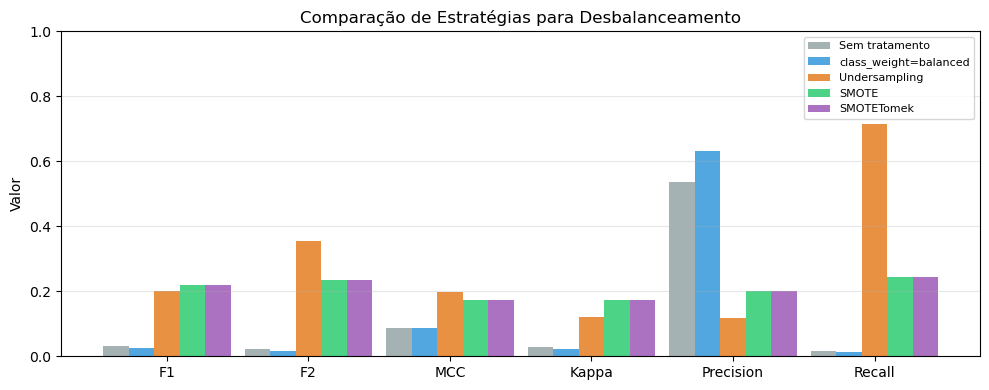
\includegraphics[width=\columnwidth]{figs/rf/fig_estrategias_comp.png}\\[3pt]
  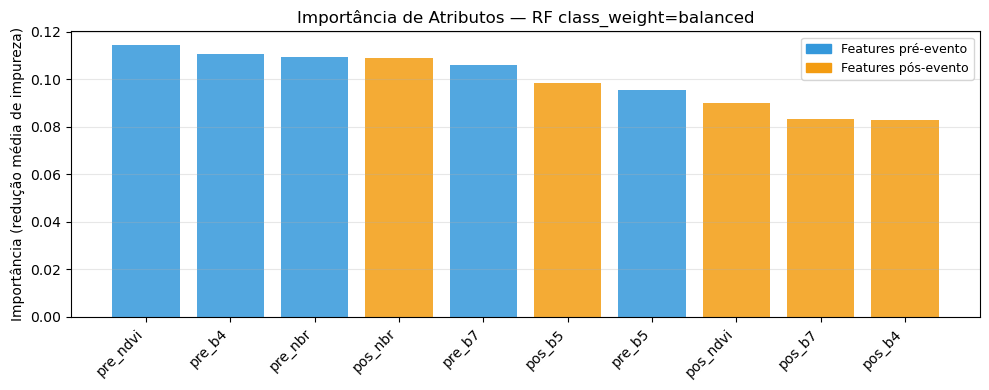
\includegraphics[width=\columnwidth]{figs/rf/fig_importancia.png}
  \caption{RF: comparação de estratégias por métrica (cima) e
           importância de atributos — distribuição uniforme 8,3\%--11,5\%
           confirma ausência de leakagem (baixo).}
  \label{fig:rf}
\end{figure}

\subsubsection{Validação Cross-Cena}

O modelo treinado em 221/074 e aplicado diretamente em 220/075 obteve
$F_2 = 0{,}472$ e AUPRC~$= 0{,}467$, superiores à validação intra-cena
($F_2 = 0{,}395$, AUPRC~$= 0{,}260$) — resultado encorajador que confirma
generalização entre órbitas e entre os sensores Landsat~8 e~9.

\subsection{Comparação Geral}

A Tabela~\ref{tab:comparacao} consolida os resultados. As diferenças de
protocolo limitam a comparação direta; os valores devem ser interpretados
com cautela.

\begin{table}[!t]
  \caption{Comparação geral — todos os modelos}
  \label{tab:comparacao}
  \centering
  \setlength{\tabcolsep}{3pt}
  \begin{tabular}{llcccc}
    \toprule
    \textbf{Modelo} & \textbf{Cena Teste} & \textbf{Recall}
                    & \textbf{Prec.} & \textbf{F1} & \textbf{AUC} \\
    \midrule
    KNN (interno)   & intra-cena 30\%    & 0,77 & 0,71 & 0,74 & —     \\
    KNN (nova cena) & cena indep.        & 0,82 & 0,09 & 0,17 & —     \\
    SVM Linear      & 222/074            & 0,83 & 0,14 & 0,24 & —     \\
    SVM RBF         & 221/074 (cego)     & 1,00 & 0,99 & \textbf{0,991} & 1,000 \\
    SVM RBF         & 222/074 (cego)     & 0,99 & 0,97 & \textbf{0,981} & 1,000 \\
    MLP (CV média)  & 220/075+221/074    & 0,69 & 0,75 & 0,722 & 0,812 \\
    MLP (cego)      & 222/074 (40M~px)   & 0,71 & 0,12 & 0,199 & 0,830 \\
    SOM$^\dagger$   & 221/074            & —    & —    & —     & —     \\
    RF (intra)      & 221/074 (blocos)   & 0,60 & 0,17 & \multicolumn{2}{c}{$F_2=0{,}395$} \\
    RF (cross)      & 220/075            & 0,66 & 0,22 & \multicolumn{2}{c}{$F_2=0{,}472$} \\
    \bottomrule
    \multicolumn{6}{l}{$^\dagger$SOM sem métricas externas: QE=0,572,
      TE=0,133, Sil.=0,341.}
  \end{tabular}
\end{table}

%=====================================================================
\section{Discussão}

\subsection{Leakage Circular e Validade Metodológica}

O experimento RF demonstrou o impacto silencioso do leakage: com dNBR
e dNDVI como atributos, $F_2 = 1{,}000$ e Kappa~$= 1{,}000$ em todas
as estratégias — resultado impossível para um problema com fronteira
espectral ambígua. Após a remoção, as métricas caíram para intervalos
realistas ($F_2 \in [0{,}02,\,0{,}47]$) e a importância distribuiu-se
uniformemente. A análise de importância de atributos é a principal
ferramenta de diagnóstico para esse tipo de vício.

O KNN usa dNBR, dNBRSWIR e dNDVI como atributos — índices de diferença
temporal que, embora não derivados diretamente da mesma máscara, tornam
o modelo dependente da calibração radiométrica relativa entre datas.
Isso explica parte da degradação ao generalizar para nova cena com
condições de aquisição distintas.

\subsection{Protocolo de Validação}

A disparidade entre SVM~RBF ($F_1 > 98\%$) e RF ($F_2 \approx 0{,}40$)
reflete, em parte, os protocolos distintos: a SVM~RBF foi avaliada em
imagens inteiras sem restrição geográfica; o RF usou blocos espaciais —
mais conservador e mais próximo da realidade de generalização. O MLP
ilustra o efeito do desbalanceamento no teste: treinar com 50/50 e
testar em 97:3 com threshold~$= 0{,}5$ produz AUC alto (0,830) mas
Precision baixa (11,6\%) — ajuste de limiar via curva PR resolveria.

\subsection{Atributos e Generalização}

A progressão SVM~Linear (2~feats, $F_1=24\%$) $\to$ SVM~RBF (10~feats,
$F_1 > 98\%$) evidencia o ganho ao incorporar B4, B5, B7 e NBR além do
NDVI. No RF, todos os 10~atributos contribuem de forma uniforme, com
os pré-evento liderando marginalmente — o estado da vegetação antes do
incêndio é mais discriminativo que o estado pós-evento isolado. A SOM,
com 7~atributos incluindo $\Delta$NDVI e $\Delta$NBR, detectou
cicatrizes sem supervisão com resultado espacialmente coerente.

%=====================================================================
\section{Conclusão}

Este trabalho comparou seis algoritmos para detecção de área queimada em
Landsat~8/9, enfatizando os aspectos metodológicos que condicionam a
validade dos resultados:

\begin{enumerate}
  \item \textbf{SVM~RBF} — melhor desempenho absoluto nos testes cegos
        ($F_1 > 98\%$, AUC-ROC~$= 1{,}000$) com 105~vetores de suporte.
  \item \textbf{RF + blocos espaciais} — avaliação mais rigorosa
        ($F_2 = 0{,}472$ cross-cena); importância uniforme confirma
        ausência de leakagem.
  \item \textbf{MLP} — boa separabilidade probabilística
        (AUC~$= 0{,}830$), mas degradação por desbalanceamento com
        threshold fixo.
  \item \textbf{SOM} — $\approx$154~mil ha detectados sem rótulos;
        adequada para triagem exploratória.
  \item \textbf{SVM~Linear} — Recall~$= 83\%$ com apenas 2~atributos;
        Precision baixa indica necessidade de atributos adicionais.
  \item \textbf{KNN} — 73\% internamente, mas 9\% de Precision em nova
        cena; fraca generalização espacial.
  \item \textbf{Leakage circular} é crítico: dNBR como feature inflou
        todas as métricas para valores perfeitos e artificiais.
\end{enumerate}

Trabalhos futuros: padronizar protocolos de validação para comparação
justa; adotar máscara independente (MapBiomas~\cite{b6}) para
reintroduzir dNBR/dNDVI; avaliar XGBoost e LightGBM; e estender a
avaliação para múltiplas cenas, anos e biomas.

%=====================================================================
\begin{thebibliography}{00}

\bibitem{b1}
P.~M.~Brando \textit{et al.},
``Abrupt increases in Amazonian tree mortality due to drought–fire
interactions,''
\textit{Proc. Natl. Acad. Sci.}, vol.~111, pp.~6347--6352, 2014.

\bibitem{b2}
C.~H.~Key e N.~C.~Benson,
``Landscape Assessment: Composite Burn Index,''
in \textit{FIREMON}, USDA Forest Service, RMRS-GTR-164-CD, 2006.

\bibitem{b3}
L.~Breiman,
``Random Forests,''
\textit{Machine Learning}, vol.~45, pp.~5--32, 2001.

\bibitem{b4}
H.~Karasiak \textit{et al.},
``Spatial dependence between training and test sets: another pitfall of
classification accuracy assessment in remote sensing,''
\textit{Machine Learning}, vol.~111, pp.~2715--2740, 2022.

\bibitem{b5}
N.~V.~Chawla \textit{et al.},
``SMOTE: Synthetic Minority Over-sampling Technique,''
\textit{J. Artif. Intell. Res.}, vol.~16, pp.~321--357, 2002.

\bibitem{b6}
MapBiomas Project,
``MapBiomas Annual Mapping of Land Use and Land Cover in Brazil,''
\texttt{https://mapbiomas.org}, 2024.

\bibitem{b7}
C.~Cortes e V.~Vapnik,
``Support-vector networks,''
\textit{Machine Learning}, vol.~20, pp.~273--297, 1995.

\bibitem{b8}
T.~Kohonen,
``Self-organized formation of topologically correct feature maps,''
\textit{Biological Cybernetics}, vol.~43, pp.~59--69, 1982.

\bibitem{b9}
Y.~LeCun, Y.~Bengio e G.~Hinton,
``Deep learning,''
\textit{Nature}, vol.~521, pp.~436--444, 2015.

\bibitem{b10}
J.~Bergstra \textit{et al.},
``Algorithms for hyper-parameter optimization,''
\textit{NeurIPS}, vol.~24, pp.~2546--2554, 2011.

\end{thebibliography}

\end{document}
